% =====================================================================
%  c22 —— 原文印刷页 172–181（PDF 第 173–182 页）
%  含：B.2 推广：Berezin-Toeplitz 量子化（及 B.2.1 球面的量子化与 SU(2) 的表示）、
%      B.3 Borel-Weil-Bott 定理、附录 C 关于 SL(2,Z) 的一些细节（C.1、C.2）；
%      插图 Fig. 32（钥匙孔区域）。
% =====================================================================

\subsection{推广：Berezin-Toeplitz 量子化} % 原文: B.2 Generalization: Berezin-Toeplitz Quantization

% 本片段中 B.2、B.3 均为 \subsection 级（节级标题 B. 在前一片段 c21 中），
% 按规范「本节重点」只加在 \section 开头，故这两个小节的要点记在此处备忘：
% (i) 适用条件：相空间除辛结构外还带有相容的复结构 $J$（使 $\omega$ 成为正的 $(1,1)$ 形式），
%     且 $\omega$ 可取为全纯线丛 $L$ 上 Hermitian 联络的曲率，于是几何量子化化为
%     「全纯截面空间 $\mathcal{H}_\kappa=\ker\bar\partial$ 加 $L^2$ 内积」，$\hbar=1/\kappa$；
% (ii) 量子化映射 $Q^{(\kappa)}(f)=\Pi\circ M_f\circ\iota$，矩阵元见 (B.20)；
% (iii) 辛体积有限 $\Rightarrow$ 有限维 $\mathcal{H}$；把 $\omega/2\pi$ 认作 $c_1(\mathcal{L})$，
%     指标公式 (B.24)（Hirzebruch--Riemann--Roch）在 $\mathcal{L}$ 充分正、高阶上同调消没时给出精确维数，
%     其 $k\to\infty$ 展开 (B.25) 首项即「每 $2\pi\hbar$ 体积一个态」的 Bohr--Sommerfeld 规则，
%     下一阶符号由 $c_1(T^{1,0}\mathcal{P})$ 决定（正曲率增加、负曲率减少量子态数）；
% (iv) 范例 $S^2=\mathbb{CP}^1=SU(2)/U(1)$：取 $K=\log(1+|z|^2)$ 时 $\mathcal{H}_\kappa$ 为 $\kappa+1$ 维，
%     即 $\mathbf{su}(2)$ 的自旋 $j=\kappa/2$ 不可约表示，而辛体积给出的是 $2j$。

当相空间额外带有 Kähler 流形的结构时，有一种非常漂亮的量子化程序可用，它在 Chern-Simons 理论中极其有用。关于 Berezin-Toeplitz 量子化的描述，可参见例如 [53] 及其所引文献。

回忆一下：辛流形是 Kähler 流形，是指它带有一个 Riemann 度量
\begin{equation}
  ds^2=g_{\mu\nu}du^\mu du^\nu\qquad\qquad \mu,\nu=1,\dots,2n.
  \tag{B.7}
  \label{eq:B.7}
\end{equation}
以及一个与度量相容的复结构，使得辛形式是一个正的 $(1,1)$ 形式，即
\begin{equation}
  \omega(v_1,Jv_2)=g(v_1,v_2)
  \tag{B.8}
  \label{eq:B.8}
\end{equation}
% [Tutor Note: (B.8) 的第二个自变量是 $Jv_2$ 而不是 $Jv_1$：由 $g$ 对称、$\omega$ 反对称可直接推出 $J$ 与 $g$ 相容（$g(Jv_1,Jv_2)=g(v_1,v_2)$）以及 $\omega$ 是 $(1,1)$ 型。若把 (B.8) 记成 $\omega(Jv_1,v_2)=g(v_1,v_2)$，则与 (B.11) 的 $\omega_{\mu\lambda}J_\nu^{\ \lambda}=g_{\mu\nu}$ 相差一个整体符号——核对时用 (B.11) 的指标形式最省事]

用局部坐标写出来，这意味着在局部坐标下辛形式一般取如下形式
\begin{equation}
  \omega=\frac{1}{2}\omega_{\mu\nu}dx^\mu\wedge dx^\nu
  \tag{B.9}
  \label{eq:B.9}
\end{equation}
Poisson 括号：
\begin{equation}
  \{f_1,f_2\}=\omega^{\mu\nu}\frac{\partial f_1}{\partial x^\mu}\frac{\partial f_2}{\partial x^\nu}
  \tag{B.10}
  \label{eq:B.10}
\end{equation}
以及
\begin{equation}
  \omega_{\mu\lambda}J_\nu^{\ \lambda}=g_{\mu\nu}
  \tag{B.11}
  \label{eq:B.11}
\end{equation}
其中复结构为
\begin{equation}
  J\Big(\frac{\partial}{\partial u^\mu}\Big)=J_\mu^{\ \nu}\frac{\partial}{\partial u^\nu}
  \tag{B.12}
  \label{eq:B.12}
\end{equation}
% [Tutor Note: 这里三处指标的上下位置最易抄错：(B.10) 用的是 $\omega$ 的\emph{逆矩阵} $\omega^{\mu\nu}$（不是 $\omega_{\mu\nu}$），否则 Poisson 括号的指标缩并就写不出来；(B.11) 中 $J_\nu^{\ \lambda}$ 的第一个指标在下、第二个在上，表示 $J$ 作为 $(1,1)$ 型张量；(B.12) 中 $J_\mu^{\ \nu}$ 的指标次序与 (B.11) 必须一致，才能由 $\omega_{\mu\lambda}J_\nu^{\ \lambda}=g_{\mu\nu}$ 反解出 $J$。原文把 $\omega^{\mu\nu}$ 与 $\omega_{\mu\nu}$ 混排版，转写时按上下文取逆]

存在局部复坐标 $z^i$，使得我们可以写
\begin{equation}
  ds^2=\frac{1}{2}g_{i\bar j}dz^i\otimes d\bar z^{\bar j}+cplx.conj.\qquad\qquad i,j=1,\dots,n.
  \tag{B.13}
  \label{eq:B.13}
\end{equation}
其中 $g_{i\bar j}$ 是 Hermitian 度量
\begin{equation}
  (g_{i\bar j})^*=g_{j\bar i}
  \tag{B.14}
  \label{eq:B.14}
\end{equation}
而在这些坐标下辛形式为
\begin{equation}
  \omega=\frac{i}{2}g_{i\bar j}dz^id\bar z^{\bar j}
  \tag{B.15}
  \label{eq:B.15}
\end{equation}

可以验证它是一个实形式。Kähler 势（的一种选择）是一个局部定义的函数，使得
\begin{equation}
  \omega=i\partial\bar\partial K
  \tag{B.16}
  \label{eq:B.16}
\end{equation}
{\small\itshape ［原文标记：此处缺少归一化因子！！！！］}
% [原文待办标记，原文 p.172 右侧边注；原文写作 "MISSING NORMALIZAATION FACTOR HERE!!!!"（NORMALIZAATION 为原文拼写笔误）]
% [Tutor Note: 作者自己标出 (B.16) 缺归一化因子，这一处确实致命：若取 $\omega=\frac{i}{2\pi}\partial\bar\partial K$（文献中更常见），则 (B.29) 的 $\int_{\mathbb{CP}^1}\omega/2\pi=+1$ 与 (B.30) 的 $h=(1+|z|^2)^{-\kappa}$ 才同时成立；若照 (B.16) 的字面取 $\omega=i\partial\bar\partial K$，则 $K=\log(1+|z|^2)$ 给出的是 $2\pi\omega_{\text{标准}}$，全部 $L^2$ 内积 (B.19)、(B.30)、(B.31) 都要相应改动。下文 (B.29) 的结果表明作者实际使用的是带 $1/2\pi$ 的约定]

我们现在假定存在全纯线丛 $L\to\mathcal{P}$，带有 Hermitian 度量 $h$ 以及与度量相容的联络 $\nabla$，使得其曲率 $F(\nabla)=\omega$。于是我们可以定义
\begin{equation}
  \mathcal{H}_\kappa:=\ker\big[\bar\partial:\Omega^{0,0}(L^{\otimes\kappa})\to\Omega^{0,1}(L^{\otimes\kappa})\big]
  \tag{B.17}
  \label{eq:B.17}
\end{equation}

这里 $\Omega^{p,q}(L^{\otimes\kappa})$ 是 $L^{\otimes\kappa}$ 的整体定义的 $\mathcal{C}^\infty$ 截面（取值于 $\mathcal{P}$ 上的 $(p,q)$ 形式）所构成的内积空间。我们把 $\mathcal{H}_\kappa$ 看作 $\Omega^{0,0}(L^{\otimes\kappa})$ 的 Hilbert 空间完备化的一个子空间。代数 $\mathcal{C}(X)$ 的 Berezin-Toeplitz 量子化是映射 $f\mapsto Q^{(\kappa)}(f)$，其中
\begin{equation}
  Q^{(\kappa)}(f):=\Pi\circ M_f\circ\iota
  \tag{B.18}
  \label{eq:B.18}
\end{equation}

这里 $\iota:\mathcal{H}_\kappa\hookrightarrow\Omega^{0,0}(L^{\otimes\kappa})$ 是包含映射，$M_f$ 是 Hilbert 空间 $\Omega^{0,0}(L^{\otimes\kappa})$ 上的乘法算符，而 $\Pi$ 是到闭子空间 $\mathcal{H}_\kappa$ 的正交投影。两个全纯截面的内积为
\begin{equation}
  \langle s_1,s_2\rangle=\int_X h^\kappa(s_1,s_2)\frac{\omega^n}{n!}
  =\int_X e^{-\kappa K}s_1(x)^*s_2(x)\prod_i\frac{d\bar z_idz_i}{2\pi i}
  \tag{B.19}
  \label{eq:B.19}
\end{equation}

按这个内积，函数 $f$ 的量子化 \eqref{eq:B.18} 就是矩阵元为
\begin{equation}
  \langle s_1,Q^{(\kappa)}(f)s_2\rangle=\int_X e^{-\kappa K}s_1(x)^*f(x)s_2(x)\prod_i\frac{d\bar z_idz_i}{2\pi i}
  \tag{B.20}
  \label{eq:B.20}
\end{equation}
的算符。{\small\itshape ［原文标记：归一化因子——$\pi$ 的因子］}
% [原文待办标记，原文 p.173 右侧边注；原文写作 "NORMALIZATION FACTORS: FACTORS OF π"]

{\small\itshape ［原文标记：GENERAL COHERENT STATES（一般相干态）］}
% [原文待办标记，原文 p.173；作者以全大写占位，提示此处应补写「一般相干态」一小节的内容（下面的评注 1–4 即该小节的素材）]

\textbf{评注：}

\begin{enumerate}
  \item 我们可以把 $L^{\otimes\kappa}$ 的一个截面 $s$ 看作定义在坐标卡 $\mathcal{U}_\alpha$ 上的一族复值函数 $s_\alpha(x)$（各 $\mathcal{U}_\alpha$ 构成 $X$ 的一个图册），使得当 $x\in\mathcal{U}_\alpha\cap\mathcal{U}_\beta$ 时
  \begin{equation}
    s_\alpha(x)=(g_{\alpha\beta}(z))^\kappa s_\beta(x)
    \tag{B.21}
    \label{eq:B.21}
  \end{equation}
  其中 $g_{\alpha\beta}(z)$ 是全纯转移函数。于是 $e^{-\kappa K}|s|^2$ 是 $X$ 上良定义的函数，即在卡的重叠处有
  \begin{equation}
    e^{-\kappa K^{(\alpha)}}|s_\alpha(x)|^2=e^{-\kappa K^{(\beta)}}|s_\beta(x)|^2
    \tag{B.22}
    \label{eq:B.22}
  \end{equation}
  这是因为在我们所用的平凡化下，$K$ 按 Kähler 变换改变：
  \begin{equation}
    K^{(\alpha)}=K^{(\beta)}+\log g_{\alpha\beta}(z)+\overline{\log g_{\alpha\beta}(z)}
    \tag{B.23}
    \label{eq:B.23}
  \end{equation}

  \item 大 $k$ 时，每 $2\pi\hbar$ 单位体积有一个态。这不过是 Bohr--Sommerfeld 半经典量子化规则。特别地，若相空间具有有限的辛体积，则存在有限维的态 Hilbert 空间。

  \item 在好的情形下，当 $\mathcal{L}$ 充分正时，$i>0$ 的 $H^i(\mathcal{P},\mathcal{L}^{\otimes k})$ 会为零，于是可以用指标公式算出 Hilbert 空间的精确维数：
  \begin{equation}
    \dim_{\mathbb{C}}H^0(\mathcal{P};\mathcal{L}^{\otimes k})=\int_{\mathcal{P}}e^{kc_1(\mathcal{L})}Td(T^{1,0}\mathcal{P})
    \tag{B.24}
    \label{eq:B.24}
  \end{equation}
  由于 $c_1(\mathcal{L})$ 由 $\frac{\omega}{2\pi}$ 代表，故 $k\to\infty$ 时可写成
  \begin{equation}
    \dim_{\mathbb{C}}H^0(\mathcal{P};\mathcal{L}^{\otimes k})
    =k^n\mathrm{vol}\,(\mathcal{P})\Big(1+\frac{n\pi}{k}\frac{\int_{\mathcal{P}}\omega^{n-1}c_1(T^{1,0}\mathcal{P})}{\int_{\mathcal{P}}\omega^n}+\mathcal{O}(k^{-2})\Big)
    \tag{B.25}
    \label{eq:B.25}
  \end{equation}
  其中 $\mathrm{vol}\,(\mathcal{P}):=\int_{\mathcal{P}}\frac{1}{n!}\big(\frac{\omega}{2\pi}\big)^n$，而 $\dim_{\mathbb{R}}\mathcal{P}=2n$。

  回想 $\hbar=1/k$，我们便看到：
  % [Tutor Note: (B.24) 是 Hirzebruch--Riemann--Roch 定理（即 $\bar\partial$ 的 Atiyah--Singer 指标定理）的截面形式：$H^0-H^1+\cdots=\int e^{kc_1}\mathrm{Td}$。作者写 "In good cases ... will vanish for $i>0$"，省略的正是 Kodaira 消没定理（$\mathcal{L}$ 充分正 $\Rightarrow H^i(\mathcal{P},\mathcal{O}(\mathcal{L}))=0$，$i>0$），没有它 (B.24) 只给出 Euler 示性数而非 $\dim H^0$。由 (B.24) 到 (B.25) 还用了 $\mathrm{Td}=1+\frac{1}{2}c_1(T^{1,0}\mathcal{P})+\cdots$ 与 $\mathrm{ch}(\mathcal{L}^k)=e^{kc_1}$，并把 $\int\omega^n$ 的 $n!$ 与 $\mathrm{vol}$ 的定义对齐]

  \item 半经典结果有一系列 $\hbar=1/k$ 的有限阶修正。其符号取决于 $c_1(T^{1,0}\mathcal{P})$ 的符号。一般而言，曲率会改变半经典的期望。大 $k$ 时，正曲率为更多的量子态腾出空间，负曲率则消灭量子态。
\end{enumerate}

\subsubsection{例：球面的量子化与 $SU(2)$ 的表示} % 原文: B.2.1 Example: Quantization Of The Sphere And Representations Of SU(2)

商 $SU(2)/U(1)$ 是余伴随轨道（coadjoint orbit）的一个例子，在带穿孔的曲面上量子化 Chern-Simons 理论时正需要对它作量子化。一般而言，$G/T$ 可以赋予 Kähler 流形的结构，而 Kähler 量子化很适于处理这个问题。

Hopf 纤维化 $\pi:SU(2)\to S^2$ 表明 $S^2\cong SU(2)/U(1)$。通过把 $S^2$ 与 $\mathbb{CP}^1$ 等同，我们也可以给它一个自然的复结构。用球极投影（stereographic projection）投到复平面来具体描述是很有用的。基本公式如下：
\begin{equation}
  \begin{aligned}
    z&=\frac{x_1+ix_2}{1+x_3}=e^{i\phi}\tan\Big(\frac{\theta}{2}\Big)\\
    \frac{z}{1+|z|^2}&=\frac{1}{2}(x_1+ix_2)=e^{i\phi}\sin\theta\\
    \frac{1}{1+|z|^2}&=\cos^2(\theta/2)=\frac{1+\cos\theta}{2}\\
    \frac{-i\,dz\wedge d\bar z}{(1+|z|^2)^2}&=\frac{1}{2}\sin\theta\, d\phi\wedge d\theta
  \end{aligned}
  \tag{B.26}
  \label{eq:B.26}
\end{equation}
其中 Bott 投影算子为
\begin{equation}
  \frac{1}{2}(1+\hat x\cdot\vec\sigma)=\frac{1}{1+|z|^2}
  \begin{pmatrix}
    |z|^2 & \bar z\\
    z & 1
  \end{pmatrix}
  \tag{B.27}
  \label{eq:B.27}
\end{equation}
% [Tutor Note: (B.27) 左端是 $S^2\subset\mathbb{R}^3$ 到 $\mathbb{CP}^1$ 上的秩一投影（Bott 投影算子），$\hat x$ 是单位向量、$\vec\sigma$ 是 Pauli 矩阵。核对方法：取 $\hat x=(0,0,1)$ 即 $z=0$，右端退化为 $\mathrm{diag}(0,1)$，与 $\frac{1}{2}(1+\sigma_3)$ 相符；若把 (B.27) 中 $z$ 与 $\bar z$ 的位置互换（即取相反的复结构），则 (B.28) 的 $\omega$ 与 (B.29) 的体积符号都会反号]

球极投影后的辛形式为
\begin{equation}
  \frac{\omega}{2\pi}=\frac{i}{2\pi}\frac{dz\wedge d\bar z}{(1+|z|^2)^2}=\frac{1}{2\pi i}\partial\bar\partial\log(1+|z|^2)
  \tag{B.28}
  \label{eq:B.28}
\end{equation}
注意辛体积为
\begin{equation}
  \int_{\mathbb{CP}^1}\frac{\omega}{2\pi}=+1
  \tag{B.29}
  \label{eq:B.29}
\end{equation}

我们可以取 Kähler 势 $K=\log(1+|z|^2)$。注意它在 $\mathbb{CP}^1$ 上不是单值的：如果取坐标为 $w=1/z$ 的另一个球极投影，我们就会用 $K=\log(1+|w|^2)=\log(1+|z|^2)-\log z-\log\bar z$。

Hopf 线丛带有 Hermitian 度量，因此若把 $L$ 的截面看作 $\mathbb{C}$ 上的函数，它们就不过是 $\mathbb{C}$ 上在无穷远处增长受限的复值函数。纤维 $L_x^{\otimes\kappa}$ 上的 Hermitian 内积由下式给出：
\begin{equation}
  h(\psi_1(x),\psi_2(x)):=(1+|z|^2)^{-\kappa}\psi_1^*(x)\psi_2(x)=e^{-\kappa K}\psi_1^*(x)\psi_2(x)
  \tag{B.30}
  \label{eq:B.30}
\end{equation}
从而 $\Gamma(L^{\otimes\kappa})$ 上的内积为
\begin{equation}
  \langle\psi_1,\psi_2\rangle=\int_{\mathbb{C}}h(\psi_1(x),\psi_2(x))\frac{\omega}{2\pi}
  =\frac{i}{2\pi}\int_{\mathbb{C}}\frac{1}{(1+|z|^2)^{\kappa+2}}\psi_1^*(x)\psi_2(x)dz\wedge d\bar z
  \tag{B.31}
  \label{eq:B.31}
\end{equation}

可归一化的函数必须满足 $\psi(z,\bar z)\sim r^\ell$，其中 $\ell<\frac{1}{2}(\kappa+1)$。

在几何量子化中，Hilbert 空间 $\mathcal{H}_\kappa=Hol(L^{\otimes\kappa})$ 是 $\kappa+1$ 维的。注意它是有限维的，因为辛空间的体积有限。事实上，若定义算符
\begin{equation}
  J^i:=(j+1)Q^{(\kappa)}(x^i)
  \tag{B.32}
  \label{eq:B.32}
\end{equation}
其中 $j:=\kappa/2$，而 $x^i$ 是把 $S^2$ 视为 $\mathbb{R}^3$ 中单位球面时 $\mathbb{R}^3$ 上标准坐标函数在 $S^2$ 上的限制，则会发现 $J^i$ 满足 $\mathbf{su}(2)$ 的标准对易关系：
\begin{equation}
  [J^i,J^j]=i\epsilon^{ijk}J^k
  \tag{B.33}
  \label{eq:B.33}
\end{equation}
事实上，$\mathcal{H}_\kappa$ 就是 $\mathbf{su}(2)$ 的自旋 $j=\kappa/2$ 的不可约表示。{\small\itshape ［原文标记：这个对易关系里的符号对不对？］}
% [原文待办标记，原文 p.175 右侧边注，位于 (B.33) 与 (B.34) 之间；原文写作 "SIGN IN THIS COMMUTATOR ?"]
注意辛体积
\begin{equation}
  \int_{\mathbb{CP}^1}\frac{\omega^{(\kappa)}}{2\pi}=\kappa=2j
  \tag{B.34}
  \label{eq:B.34}
\end{equation}
并不是 Hilbert 空间的精确维数，后者是 $\kappa+1=2j+1$。二者只在半经典极限 $\kappa\to\infty$ 下相符。
% [Tutor Note: 作者自己在边注里怀疑 (B.33) 的符号。正确读法是：$x^i$ 是 $\mathbf{su}(2)^*$ 上的坐标函数，满足 $\{x^i,x^j\}=\epsilon^{ijk}x^k$；几何量子化把 Poisson 括号送到 $\frac{1}{i\hbar}[\cdot,\cdot]$，而这里 $\hbar=1/(j+1)$，故 $[Q(x^i),Q(x^j)]=i\epsilon^{ijk}Q(x^k)/(j+1)$，再乘上 (B.32) 的因子 $j+1$ 即得 (B.33) 的 $+i\epsilon^{ijk}J^k$。(B.33) 本身无误，作者的疑问来自 $j+1$ 这个看似多余的归一化（它保证 $\omega^{(\kappa)}=2j$ 而 $\dim\mathcal{H}_\kappa=2j+1$）；若把 (B.32) 的 $j+1$ 误读成 $j$，就会以为右端差一个符号]

\subsection{Borel-Weil-Bott 定理} % 原文: B.3 The Borel-Weil-Bott Theorem

% 本小节（\subsection 级）按规范不加「本节重点」；要点备忘：
% (i) 上一小节的 $S^2=SU(2)/U(1)$ 只是特例：Borel-Weil-Bott 定理把「齐性空间上的全纯线丛截面」
%     与「$G$ 的不可约表示」一般地对应起来，$G/T=G^{\mathbb{C}}/P$ 既紧又是 Kähler（旗流形）；
% (ii) 辛结构来自余伴随轨道 $\mathcal{O}(\lambda)\subset\mathbf{g}^*$，$\omega_\lambda(X,Y)=\frac12\langle\lambda,[X,Y]\rangle$
%     是 Kirillov--Kostant--Souriau 形式，在轨道切空间上非退化；
% (iii) 用不变双线性型等同 $\mathbf{g}\cong\mathbf{g}^*$ 后可写成 $\omega_{t_0}(X,Y)=\frac12\operatorname{tr}(t_0[X,Y])$，
%     这正是讨论 Chern-Simons 理论时使用的形式；
% (iv) 两种读法：数学读法为全纯线丛截面/诱导表示，物理读法为相空间路径积分（并有 SQM 实现）。

前面那个例子是一个更一般、也更漂亮的定理——Borel-Weil-Bott 定理——的非常特殊的情形。

$G/T=G^{c}/P$，既是紧流形又是 Kähler 流形。{\small\itshape ［原文标记：需要讨论复结构与 Kähler 形式。］}
% [原文待办标记，原文 p.175；作者在此处留下两句未展开的草稿说明]
关于旗流形几何的一本好参考书：Alekseevsky。
\begin{equation}
  \mathcal{O}(\lambda)\subset\mathbf{g}^*
  \tag{B.35}
  \label{eq:B.35}
\end{equation}
% [原文标记：此处为一行星号分隔线（原稿的分段记号，无文字），原文 p.175]
仅仅用双线性型把 $\mathbf{g}\cong\mathbf{g}^*$ 作为向量空间等同起来。
% [原文标记：此处为一行星号分隔线（原稿的分段记号，无文字），原文 p.175；与上一行共同框住中间那句草稿]

辛结构族：若 $\lambda\in\mathbf{g}^*$，则
\begin{equation}
  \omega_\lambda(X,Y)=\frac{1}{2}\langle\lambda,[X,Y]\rangle
  \tag{B.36}
  \label{eq:B.36}
\end{equation}
它从 $\mathbf{g}$ 上的 2-形式下降为 $T_\lambda\mathcal{O}(\lambda)$ 上的 2-形式，并在那里变为非退化的。用 $\mathbf{g}$ 上的非退化双线性型 $\operatorname{tr}$ 可以把 $\mathbf{g}$ 与 $\mathbf{g}^*$ 等同，从而与伴随轨道等同，于是若 $t_0\in\mathbf{t}\subset\mathbf{g}$，我们也可以改写成
\begin{equation}
  \omega_{t_0}(X,Y)=\frac{1}{2}\operatorname{tr}\,(t_0[X,Y])
  \tag{B.37}
  \label{eq:B.37}
\end{equation}
这是在讨论 Chern-Simons 理论时更有用的形式。
% [Tutor Note: (B.35)–(B.37) 中原文用的是\emph{粗正体} $\mathbf{g}$、$\mathbf{t}$（而非哥特体 $\mathfrak{g}$）：这一段是草稿，字体与前文（如第 4 章的 $\mathfrak{g}$）不一致。译文按页面图像保留粗正体以忠实于原稿；若全书的记号要统一，只需把本节所有 \verb|\mathbf{g}| 换成 \verb|\mathfrak{g}|，不影响任何公式内容。另外 (B.36) 的 $\frac12$ 与 (B.37) 的 $\frac12\operatorname{tr}$ 必须同乘同一个常数，否则 $\omega_{t_0}$ 与 $\omega_\lambda$ 差一个因子 2]

数学版本：全纯线丛的截面。诱导表示。等等。
% [原文标记：此处为一长行星号分隔线（原稿的分段记号，无文字），原文 p.175]
物理版本：相空间积分。还有一种超对称量子力学（SQM）的解释。

\begin{enumerate}
  \item Alekseev、Faddeev、Shatashvili [1]
  \item Alvarez、Singer、Windey [2][3]
  \item Stone……
  \item Szabo [57]
\end{enumerate}

\begin{figure}[htbp]
  \centering
  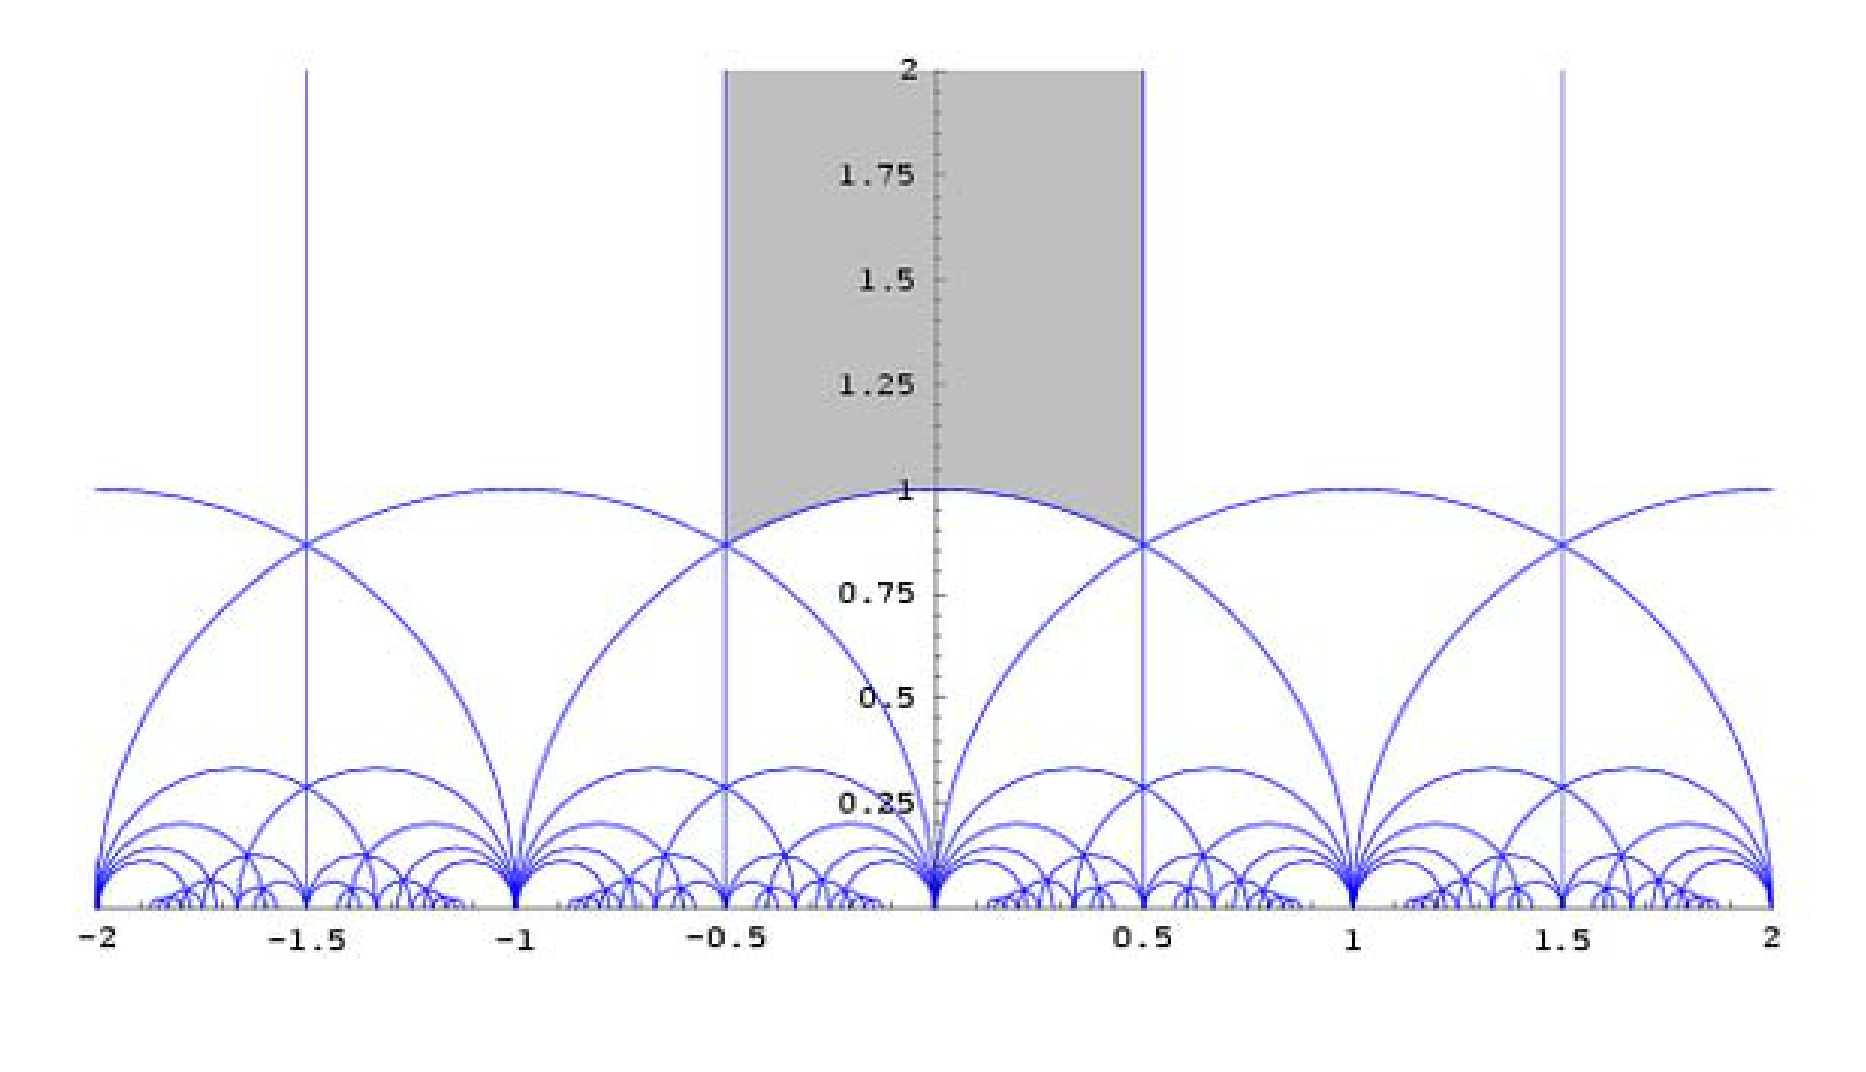
\includegraphics[width=0.78\textwidth]{figures/fig32.png}
  \caption{钥匙孔区域（keyhole region），即 $PSL(2,\mathbb{Z})$ 作用在复上半平面上的标准基本域选择。图取自维基百科「Modular Group」条目。（原文 Fig.~32，第 176 页）}
  \label{fig:32}
\end{figure}

\section{关于 $SL(2,\mathbb{Z})$ 的一些细节} % 原文: C. A Few Details About SL(2, Z)

\begin{keytakeaways}
  \item 模群 $PSL(2,\mathbb{Z}):=SL(2,\mathbb{Z})/\{\pm1\}$ 通过分式线性变换 $\tau\mapsto\frac{a\tau+b}{c\tau+d}$ 有效作用在复上半平面 $\mathcal{H}$ 上；它由 $S=\begin{pmatrix}0&-1\\1&0\end{pmatrix}$ 与 $T=\begin{pmatrix}1&1\\0&1\end{pmatrix}$ 生成。
  \item 关系只有 $S^2=-1$、$(ST)^3=(TS)^3=-1$（及其推论）。$S$ 的符号必须小心：换号后 $(ST)^3$ 变成 $+1$，但 $\bar S\in PSL$ 与符号无关。
  \item 基本域是钥匙孔区域 $\tilde{\mathcal{F}}=\{\tau\in\mathcal{H}:|\tau|\ge1,\ |\operatorname{Re}\tau|\le\frac12\}$（图 32）。证明分两步：引理 1 处理边界上的等距点（核心是配方估计 (C.8)），引理 2 列出三个有非平凡稳定化子的椭圆点 $i,\omega,-\omega^2$。
  \item 构造性算法：对 $(A,C)$ 作辗转相除法得连分数系数 $q_1,\dots,q_{N+1}$，把每步写成矩阵方程 (C.17)--(C.20)，再用 $\sigma^1\sigma^3=S$ 把 $\det\tilde g=(-1)^{N+1}$ 修正为 $SL(2,\mathbb{Z})$ 元素，最终得 $h=g^{-1}T^n$ 的 $S,T$ 字表达 (C.26)--(C.27)。
\end{keytakeaways}

\subsection{生成元与 $PSL(2,\mathbb{Z})$ 的基本域} % 原文: C.1 Generators And A Fundamental Domain For PSL(2, Z)

模群是 $PSL(2,\mathbb{Z}):=SL(2,\mathbb{Z})/\{\pm1\}$，其中 $SL(2,\mathbb{Z})$ 是 $SL(2,\mathbb{R})$ 中所有矩阵元皆为整数的矩阵构成的子群。回忆该群通过
\begin{equation}
  \begin{pmatrix}
    a & b\\
    c & d
  \end{pmatrix}\cdot\tau:=\frac{a\tau+b}{c\tau+d}
  \tag{C.1}
  \label{eq:C.1}
\end{equation}
有效地作用在复上半平面 $\mathcal{H}$ 上。

我们将求出这个群作用的一个基本域，并在此过程中证明 $SL(2,\mathbb{Z})$ 由下面定义的群元 $S$ 与 $T$ 生成：
{\small\itshape ［原文标记：需要检查我们在全文中是否一直使用了自洽的 $S$ 符号约定。］}
% [原文待办标记，原文 p.176 右侧边注]

\begin{equation}
  S=\begin{pmatrix}
    0 & -1\\
    1 & 0
  \end{pmatrix}
  \tag{C.2}
  \label{eq:C.2}
\end{equation}
\begin{equation}
  T=\begin{pmatrix}
    1 & 1\\
    0 & 1
  \end{pmatrix}
  \tag{C.3}
  \label{eq:C.3}
\end{equation}
这些矩阵满足关系
\begin{equation}
  \begin{aligned}
    S^2&=-1\\
    (ST)^3&=(TS)^3=-1
  \end{aligned}
  \tag{C.4}
  \label{eq:C.4}
\end{equation}
% [Tutor Note: 注意 (C.4) 右边是 $-1$ 而非 $1$：这正是取 $S=\begin{pmatrix}0&-1\\1&0\end{pmatrix}$（而非其负号）的结果，也说明 $S,T$ 生成的是 $SL(2,\mathbb{Z})$ 而不是 $PSL(2,\mathbb{Z})$。在下文 (C.9)、(C.10) 里 $(ST)^3=-1$ 会是 $\bar S\bar T$ 阶为 3 的来源。若把 $S$ 换成 $\begin{pmatrix}0&1\\-1&0\end{pmatrix}$，则 (C.4) 变成 $S^2=-1$、$(ST)^3=(TS)^3=+1$，与作者的提醒一致]

注意，若改变 $S$ 的符号，则 $(ST)^3=(TS)^3=+1$，所以对 $S$ 的符号定义要小心一些。

把 $S,T$ 在 $PSL(2,\mathbb{Z})$ 中的像记为 $\bar S,\bar T$。注意 $\bar S$ 不依赖于 $S$ 的符号。\footnote{这里我们沿用 J.-P. Serre，《A Course in Arithmetic》，Springer GTM 7，pp.~78--79 中一个非常好的论证。}

令
\begin{equation}
  \tilde{\mathcal{F}}:=\{\tau\in\mathcal{H}\,|\,|\tau|\ge1\quad\&\quad|\operatorname{Re}(\tau)|\le\tfrac{1}{2}\}
  \tag{C.5}
  \label{eq:C.5}
\end{equation}
这差不多是模群的典范基本域，但还不完全是。它就是图 32 所示的著名的\emph{钥匙孔区域}。令 $\bar G$ 为由 $\bar S$ 与 $\bar T$ 生成的子群。我们断言 $\cup_{g\in\bar G}\,g\cdot\tilde{\mathcal{F}}$ 是整个上半平面。为证明这一点，回忆对任意 $g\in SL(2,\mathbb{Z})$ 有
\begin{equation}
  \operatorname{Im}(g\cdot\tau)=\frac{\operatorname{Im}\tau}{|c\tau+d|^2}
  \tag{C.6}
  \label{eq:C.6}
\end{equation}
现在，对任意固定的 $\tau\in\mathcal{H}$，函数 $|c\tau+d|$ 在 $SL(2,\mathbb{Z})$ 上有下界，从而在 $G$ 上有下界。事实上，把 $\tau=x+iy$ 分成实部与虚部，
\begin{equation}
  |c\tau+d|^2=(cx+d)^2+c^2y^2\ge
  \begin{cases}
    y^2 & c\ne0\\
    d^2\ge1 & c=0
  \end{cases}
  \tag{C.7}
  \label{eq:C.7}
\end{equation}
因此，对任意固定的 $\tau$，必存在群元 $g\in\bar G$，使得 $\operatorname{Im}(g\cdot\tau)$ 作为 $g$ 的函数取极大值。注意用 $\bar T$ 或 $\bar T^{-1}$ 的幂左乘 $g$ 不改变这一性质，所以使 $\operatorname{Im}(g\cdot\tau)$ 极大的 $g$ 并不唯一。我们可以用 $|\operatorname{Re}(g\cdot\tau)|\le\frac{1}{2}$ 来消去这个不确定性。选取这样的群元 $g$。我们断言：对这个变换，$\tau'=g\cdot\tau\in\tilde{\mathcal{F}}$。只需再验证 $|\tau'|\ge1$。否则 $|\tau'|<1$，但此时 $\operatorname{Im}(\bar S\cdot\tau')=\operatorname{Im}(\tau')/|\tau'|^2>\operatorname{Im}(\tau')$，与 $g$ 的定义矛盾。总之，上半平面的每个元素都可被 $\bar G$ 的适当元素带到 $\tilde{\mathcal{F}}$ 中。

现在我们需要两个引理：

\textbf{引理 1：}若 $g\in SL(2,\mathbb{Z})$ 与 $\tau$ 具有如下性质：$\tau\in\tilde{\mathcal{F}}$ 且 $g\cdot\tau\in\tilde{\mathcal{F}}$，则
\begin{enumerate}
  \item $|\operatorname{Re}(\tau)|=\frac{1}{2}$ 且 $g\cdot\tau=\tau\pm1$，或者
  \item $|\tau|=1$
\end{enumerate}

为证明这一点，注意不失一般性（WLOG）可设 $\operatorname{Im}(g\cdot\tau)\ge\operatorname{Im}\tau$。（否则作替换 $g\to g^{-1}$、$\tau\to g^{-1}\tau$。）但这个等式蕴含 $1\ge|c\tau+d|$，后者又蕴含
\begin{equation}
  \begin{aligned}
    1&\ge|c\tau+d|^2\\
    &=(cx+d)^2+c^2y^2\\
    &=c^2|\tau|^2+2cdx+d^2\\
    &\ge c^2|\tau|^2-|cd|+d^2\\
    &=c^2\Big(|\tau|^2-\frac{1}{4}\Big)+\Big(|d|-\frac{1}{2}|c|\Big)^2\\
    &\ge\frac{3}{4}c^2+\Big(|d|-\frac{1}{2}|c|\Big)^2
  \end{aligned}
  \tag{C.8}
  \label{eq:C.8}
\end{equation}

由 \eqref{eq:C.8} 我们得出：

\begin{enumerate}
  \item $(c=0,\,d=\pm1)$ \underline{或} $(c=\pm1,\,d=0,\pm1)$。
  \item 不等式取等号当且仅当 $2cdx=-|cd|$ 且 $|\tau|=1$。
\end{enumerate}

若 $c=0$ 且 $d=\pm1$，则 $g\cdot\tau=\tau\pm1$。此时显然 $|\operatorname{Re}(\tau)|=\frac{1}{2}$。若 $c=\pm1$ 且 $d=0,\pm1$，则不等式取等号，从而 $|\tau|=1$。

\textbf{引理 2：}若 $\tau\in\tilde{\mathcal{F}}$ 且 $\bar g\cdot\tau=\tau$，其中 $\bar g\in PSL(2,\mathbb{Z})$、$\bar g\ne1$，则要么
\begin{enumerate}
  \item $\tau=i$，且稳定化子群为 $\{1,\bar S\}$
  \item $\tau=\omega=e^{2\pi i/3}=-\frac{1}{2}+\frac{\sqrt{3}}{2}i$，且稳定化子群为
  \begin{equation}
    \{1,\bar S\bar T,(\bar S\bar T)^2\}
    \tag{C.9}
    \label{eq:C.9}
  \end{equation}
  \item $\tau=-\omega^2=e^{\pi i/3}=\frac{1}{2}+\frac{\sqrt{3}}{2}i$，且稳定化子群为
  \begin{equation}
    \{1,\bar T\bar S,(\bar T\bar S)^2\}
    \tag{C.10}
    \label{eq:C.10}
  \end{equation}
\end{enumerate}

特别地，对 $\tilde{\mathcal{F}}$ 中所有其余的点 $\tau$，稳定化子群是平凡群。

引理 2 很快由引理 1 推出：若 $g\tau=\tau$，则必属 $c=\pm1$ 的情形。若 $d=0$，则对某个整数 $a$ 有 $a-1/\tau=\tau$。但还必须有 $|\tau|=1$，从而 $a=\tau+\bar\tau$。既然 $a$ 是整数，很快发现要么 $a=0$ 而 $\tau=i$，要么 $a=\pm1$ 而 $\tau=\omega$ 或 $-\omega^2$。若 $d=\pm1$，则由取等条件 $2cdx=-|cd|$ 得 $x=-\frac{1}{2}d/|d|$，从而 $\tau=\omega$ 或 $=-\omega^2$。
% [Tutor Note: 这段把引理 2 归结为「$g\tau=\tau$ 且 $\tau\in\tilde{\mathcal{F}}$ 时只能取 $|c|=1$」。缺的一步是：由 $\tau=g^{-1}\tau$ 得 $c\tau^2+(d-a)\tau-b=0$，$c\ne0$ 时 $1/\tau$ 是整系数二次方程的根，$|\tau|=1$ 给 $a=\tau+\bar\tau\in\mathbb{Z}$；作者直接写「we quickly find」跳过了对 $a\in\{-1,0,1\}$（因 $|\operatorname{Re}\tau|\le\frac12$）的枚举。另外 $d=\pm1$ 时的取等条件 $2cdx=-|cd|$ 与 $|\tau|=1$ 联立才能定出 $x$，单用其一不足以定 $\tau$]

现在终于可以证明：

\textbf{定理：}$SL(2,\mathbb{Z})$ 由 $S$ 与 $T$ 生成。

\textit{证明：}令 $\tau_0$ 位于 $\tilde{\mathcal{F}}$ 的\underline{内部}。任取元素 $g\in SL(2,\mathbb{Z})$、$\bar g\ne1$。则存在元素 $g'\in\bar G$，使得 $g'g\cdot\tau_0\in\tilde{\mathcal{F}}$。而且由引理 1，该元素必在 $\tilde{\mathcal{F}}$ 的内部，从而由引理 2，在 $PSL(2,\mathbb{Z})$ 中 $g'g=1$。因此 $\bar g\in\bar G$，即 $\bar G=PSL(2,\mathbb{Z})$。此外 $S^2=-1$，故 $S$ 与 $T$ 生成 $SL(2,\mathbb{Z})$。$\spadesuit$

\begin{enumerate}
  \item 精确的基本域 $\mathcal{F}$ 必须选得使边界上没有两个不同的点彼此 $G$-相关。例如我们可以取边界中 $\operatorname{Re}(\tau)\ge0$ 的那一部分。

  \item 通过像上面那样研究可能的不动点，可以推出 $S$ 与 $T$ 上\underline{仅有}的关系是：
  \begin{equation}
    S^2=-1\qquad (ST)^3=-1
    \tag{C.11}
    \label{eq:C.11}
  \end{equation}
  （以及由它们推出的一切关系）。

  \item 给定 $g\in SL(2,\mathbb{Z})$，可以这样写出给出 $g$ 的 $S,T$ 词：对 $(a,c)$ 施用辗转相除法，并把那里的标准等式按矩阵解释。见第 1 章第 8 节。

  \item 虽然钥匙孔区域是标准的基本域，但基本域的选择并不唯一。例如，图 32 中所示的任一个像都同样可用（当然这样的区域有无穷多个）。此外，把 $\mathcal{F}\to\mathcal{F}+\epsilon$ 平移一下也仍然得到基本域。

  \item $PSL(2,\mathbb{Z})$ 在 $\mathcal{H}$ 上的作用是真不连续的（properly discontinuous），但并不完全自由。若考虑不包含上述稳定化子群的有限指数子群，则作用将是自由的，商空间将是一个漂亮的 Riemann 曲面。
\end{enumerate}

\subsection{把 $SL(2,\mathbb{Z})$ 的元素写成 $S$ 与 $T$ 的词} % 原文: C.2 Expressing Elements Of SL(2, Z) As Words In S And T

群 $SL(2,\mathbb{Z})$ 由
\begin{equation}
  S:=\begin{pmatrix}
    0 & -1\\
    1 & 0
  \end{pmatrix}
  \qquad\&\qquad
  T:=\begin{pmatrix}
    1 & 1\\
    0 & 1
  \end{pmatrix}
  \tag{C.12}
  \label{eq:C.12}
\end{equation}
生成。

下面是把任意元素
\begin{equation}
  h=\begin{pmatrix}
    A & B\\
    C & D
  \end{pmatrix}\in SL(2,\mathbb{Z})
  \tag{C.13}
  \label{eq:C.13}
\end{equation}
分解为 $S$ 与 $T$ 的词的一个算法。

首先注意下面这个简单的

\textbf{引理} 设 $h\in SL(2,\mathbb{Z})$ 如 \eqref{eq:C.13}。又设 $g\in SL(2,\mathbb{Z})$ 满足：
\begin{equation}
  g\cdot\begin{pmatrix}
    A\\
    C
  \end{pmatrix}=\begin{pmatrix}
    1\\
    0
  \end{pmatrix}
  \tag{C.14}
  \label{eq:C.14}
\end{equation}
那么
\begin{equation}
  gh=T^n
  \tag{C.15}
  \label{eq:C.15}
\end{equation}
其中 $n\in\mathbb{Z}$ 为某个整数。

现在，设 $h$ 满足 $A>C>0$。则 $(A,C)=1$，于是可用辗转相除法定义整数 $q_\ell$，$\ell=1,\dots,N+1$，其中 $N\ge1$，使得
\begin{equation}
  \begin{aligned}
    A&=q_1C+r_1 & 0&<r_1<C\\
    C&=q_2r_1+r_2 & 0&<r_2<r_1\\
    r_1&=q_3r_2+r_3 & 0&<r_3<r_2\\
    &\;\;\vdots & &\;\;\vdots\\
    r_{N-2}&=q_Nr_{N-1}+r_N & 0&<r_N<r_{N-1}\\
    r_{N-1}&=q_{N+1}r_N & &
  \end{aligned}
  \tag{C.16}
  \label{eq:C.16}
\end{equation}
且 $r_N=(A,C)=1$。（注意你可以把 $r_0$ 解释为 $C$，这在 $N=1$ 时是必要的。）现在，{\small\itshape ［原文标记：这里 $N=0$？］}
% [原文待办标记，原文 p.180 右侧边注；原文写作 "N = 0 here?"]
把辗转相除法中的第一行写成矩阵形式：
\begin{equation}
  \begin{pmatrix}
    1 & -q_1\\
    0 & 1
  \end{pmatrix}\begin{pmatrix}
    A\\
    C
  \end{pmatrix}=\begin{pmatrix}
    r_1\\
    C
  \end{pmatrix}
  \tag{C.17}
  \label{eq:C.17}
\end{equation}
我们想要方程具有可以迭代该算法的形式，所以需要较大的整数在上面。因此把恒等式改写成
\begin{equation}
  \sigma^1\begin{pmatrix}
    1 & -q_1\\
    0 & 1
  \end{pmatrix}\begin{pmatrix}
    A\\
    C
  \end{pmatrix}=\begin{pmatrix}
    C\\
    r_1
  \end{pmatrix}
  \tag{C.18}
  \label{eq:C.18}
\end{equation}

现在可以迭代此程序了。于是辗转相除法蕴含矩阵恒等式
\begin{equation}
  \tilde g\begin{pmatrix}
    A\\
    C
  \end{pmatrix}=\begin{pmatrix}
    1\\
    0
  \end{pmatrix}
  \tag{C.19}
  \label{eq:C.19}
\end{equation}
\begin{equation}
  \tilde g=(\sigma^1T^{-q_{N+1}})\cdots(\sigma^1T^{-q_1})
  \tag{C.20}
  \label{eq:C.20}
\end{equation}
现在，要应用引理我们需要 $g$ 属于 $SL(2,\mathbb{Z})$，但
\begin{equation}
  \det\tilde g=(-1)^{N+1}
  \tag{C.21}
  \label{eq:C.21}
\end{equation}
我们可以容易地修改方程以得到所需的元素 $g$。把论证分成两种情形：

\begin{enumerate}
  \item 先设 $N+1=2s$ 为偶数。于是把 $\tilde g$ 的因子两两配对，写出
  \begin{equation}
    \begin{aligned}
      (\sigma^1T^{-q_{2\ell}})(\sigma^1T^{-q_{2\ell-1}})&=(\sigma^1\sigma^3)(\sigma^3T^{-q_{2\ell}}\sigma^3)(\sigma^3\sigma^1)T^{-q_{2\ell-1}}\\
      &=-ST^{q_{2\ell}}ST^{-q_{2\ell-1}}
    \end{aligned}
    \tag{C.22}
    \label{eq:C.22}
  \end{equation}
  % [Tutor Note: (C.22) 的三步：先用 $(\sigma^3)^2=1$ 在中间插入 $\sigma^3\sigma^3$；再用 $\sigma^3T^{-q}\sigma^3=T^{q}$（共轭把 $T$ 的幂取反：$\sigma^3\begin{pmatrix}1&-q\\0&1\end{pmatrix}\sigma^3=\begin{pmatrix}1&q\\0&1\end{pmatrix}$）；最后用 $\sigma^1\sigma^3=S$（严格等式，$\sigma^1\sigma^3=\begin{pmatrix}0&-1\\1&0\end{pmatrix}$ 正是 (C.2) 的 $S$）与 $\sigma^3\sigma^1=-i\sigma^2=-S$。于是 $(\sigma^1T^{-q_{2\ell}})(\sigma^1T^{-q_{2\ell-1}})=\sigma^1T^{-q_{2\ell}}\sigma^1T^{-q_{2\ell-1}}=-ST^{q_{2\ell}}ST^{-q_{2\ell-1}}$，负号来自 $\sigma^3\sigma^1=-S$。核对时若把 $\sigma^3\sigma^1$ 误当成 $\sigma^1\sigma^3$，就会丢掉这个负号]

  其中我们用到了 $\sigma^1\sigma^3=-i\sigma^2=S$。因此我们可以写
  \begin{equation}
    \tilde g=g=(-1)^s\prod_{\ell=1}^{s}\big(ST^{q_{2\ell}}ST^{-q_{2\ell-1}}\big)
    \tag{C.23}
    \label{eq:C.23}
  \end{equation}

  \item 现在设 $N+1=2s+1$ 为奇数。于是把恒等式 \eqref{eq:C.19} 改写为
  \begin{equation}
    \sigma^1\tilde g\begin{pmatrix}
      A\\
      C
    \end{pmatrix}=\begin{pmatrix}
      1\\
      0
    \end{pmatrix}
    \tag{C.24}
    \label{eq:C.24}
  \end{equation}
  于是现在只需取
  \begin{equation}
    g=\sigma^1\tilde g=(-1)^{s+1}(ST^{-q_{2s+1}})\prod_{\ell=1}^{s}\big(ST^{q_{2\ell}}ST^{-q_{2\ell-1}}\big)
    \tag{C.25}
    \label{eq:C.25}
  \end{equation}
\end{enumerate}

因此两种情形可以统一表述为
\begin{equation}
  g=(-1)^{\lfloor\frac{N+1}{2}\rfloor}\prod_{\ell=1}^{N+1}\big(ST^{(-1)^\ell q_\ell}\big)
  \tag{C.26}
  \label{eq:C.26}
\end{equation}
% [Tutor Note: (C.26) 与 (C.23)、(C.25) 的符号核对：$N+1=2s$（偶）时 $\lfloor\frac{N+1}{2}\rfloor=s$，与 (C.23) 的 $(-1)^s$ 一致；但 $N+1=2s+1$（奇）时 $\lfloor\frac{N+1}{2}\rfloor=s$，而 (C.25) 给出的是 $(-1)^{s+1}$——两者相差一个整体符号。原文 (C.26) 照印如此，此处照原样转写未改。由于 $-1=S^2$ 是 $SL(2,\mathbb{Z})$ 的中心元，这个整体符号不改变 $h=g^{-1}T^n$ 在 $PSL(2,\mathbb{Z})$ 中的分解，但若要求 $h\in SL(2,\mathbb{Z})$ 逐元素相等，须重核这一步（疑为原稿笔误，或 (C.25) 的 $s+1$ 应为 $s$）。另外 (C.20)、(C.23)、(C.25) 中乘积的书写次序是从 $q_{N+1}$ 在左、$q_1$ 在右，读 $\prod_{\ell=1}^{N+1}$ 时须按同一约定理解]

然后我们终于可以把
\begin{equation}
  h=\begin{pmatrix}
    A & B\\
    C & D
  \end{pmatrix}=g^{-1}T^n
  \tag{C.27}
  \label{eq:C.27}
\end{equation}
写成 $S$ 与 $T$ 的词，其中 $n$ 为适当的整数。（注意 $S^2=-1$。）
{\small\itshape ［原文标记：最好给出确定 $n$ 的算法。］}
% [原文待办标记，原文 p.181 右侧边注；原文写作 "It would be good to give an algorithm for determining n."]

现在需要说明如何把一般的 $h\in SL(2,\mathbb{Z})$ 化成 $A>C>0$ 的形式，以便套用上面的公式。注意
\begin{equation}
  \begin{pmatrix}
    1 & 0\\
    m & 1
  \end{pmatrix}\begin{pmatrix}
    A & B\\
    C & D
  \end{pmatrix}=\begin{pmatrix}
    A & B\\
    C+mA & D+mB
  \end{pmatrix}
  \tag{C.28}
  \label{eq:C.28}
\end{equation}
% [Tutor Note: 原稿 (C.28) 右端矩阵的排版有缺陷：两个元素 $A$、$B$ 之间以及与 $C+mA$、$D+mB$ 之间的列分隔丢失，看起来像 $2\times2$ 矩阵里挤了「$A\ B$」「$C+mA\ D+mB$」两团。按左乘矩阵的含义，它应当是 $\begin{pmatrix}A&B\\C+mA&D+mB\end{pmatrix}$；这里按数学含义排出，特此说明]
而
\begin{equation}
  \begin{pmatrix}
    1 & 0\\
    -m & 1
  \end{pmatrix}=ST^mS^{-1}
  \tag{C.29}
  \label{eq:C.29}
\end{equation}
于是，若 $A>0$，我们可用这一操作平移 $C$，使 $0\le C<A$。若 $A<0$，可乘以 $S^2=-1$ 化到 $A>0$ 的情形。最后，若 $A=0$，则
\begin{equation}
  h=\begin{pmatrix}
    0 & \pm1\\
    \mp1 & n
  \end{pmatrix}
  \tag{C.30}
  \label{eq:C.30}
\end{equation}
而我们写
\begin{equation}
  ST^n=\begin{pmatrix}
    0 & -1\\
    1 & n
  \end{pmatrix}
  \tag{C.31}
  \label{eq:C.31}
\end{equation}
{\small\itshape ［原文标记：需要以一种更有用的方式把结果总结一下。］}
% [原文待办标记，原文 p.181 右侧边注；原文写作 "Need to summarize the result in a useful way"]
